\documentclass[preprint2]{aastex62}

\bibliographystyle{aasjournal}
\usepackage{graphicx}
\usepackage[suffix=]{epstopdf}
\usepackage{natbib}
\usepackage{amsmath}
\usepackage{url}
\usepackage{xspace}

%    Make Scientific Notation
\providecommand{\e}[1]{\ensuremath{\times 10^{#1}}}

% make the word Kepler italicized
\newcommand{\Kepler}{\textsl{Kepler}\xspace}



\begin{document}
%%%%%%%%%%%%%%%%%%%%%%
\title{Rotating Stars from \Kepler Observed with Gaia DR2}

\shorttitle{Rotating Stars from \Kepler Observed with Gaia DR2}
\shortauthors{Davenport et al.}


\correspondingauthor{James. R. A. Davenport}
\email{James.Davenport@wwu.edu}

\author{James. R. A. Davenport}
\altaffiliation{NSF Astronomy and Astrophysics Postdoctoral Fellow}
\altaffiliation{DIRAC Fellow}
\affiliation{Department of Physics \& Astronomy, Western Washington University, 516 High St., Bellingham, WA 98225, USA}
\affiliation{Department of Astronomy, University of Washington, Seattle, WA 98195, USA}


\author{Kevin R. Covey}
\affiliation{Department of Physics \& Astronomy, Western Washington University, 516 High St., Bellingham, WA 98225, USA}


 
 

%%%%%%%%%%%%%%%%%%%%%%%%%%%%%%
\begin{abstract}
We have matched the astrometric data from {\em Gaia} Data Release 2 to the sample of stars with measured rotation periods from \Kepler. Using 30,305 stars with good distance estimates, we select 16,248 as being likely main sequence single stars within a 0.5 mag region about a 1 Gyr isochrone. This removes sub-giants and unresolved binary stars from the sample.
The rotation period bimodality, originally discovered by \citet{mcquillan2013}, is recovered for stars out to 525pc, but is not detectable at further distances. 
We also find a significant width in the stellar main sequence of $M_G\sim$0.25 mag, as well as a  increase in the average rotation period correlated with the $M_G$ offset at a given color (mass). We interpret this to be the measurable change in luminosity and loss of angular momentum as stars evolve along the main sequence, which may provide a new independent test of stellar evolution and gyrochronlogy models.
This investigation represents the first step in understanding the star formation history of our solar neighborhood as traced through stellar angular momentum loss. 
\end{abstract}



%%%%%%%%%%%%%%%%%%%%%%%%%%%%%%
\section{Introduction}

The \Kepler mission \citep{borucki2010} a new era for enabling detailed study of angular momentum loss in low-mass stars. long noted as a means to possibly age-date stars (gyro), open clusters give hope that this general model works for low-mass stars
many Qs exist about details. these include Qs about initial rotation period distribution \citep[e.g.][]{barnes2010,matt2015}, the specific prescription for spin-down \citep{angus2015}, and exploring the efficiency of this angular momentum loss mechanism at old ages \citep{van-saders2016}.


one of the most compelling results from the rotation work in \Kepler is the discovery of a period bimodality. 
\citet{mcquillan2013} found bimodal feature, in M and later K stars \citep{mcquillan2014}. Davenport used Gaia DR1 to remove contamination from sub-giants and found the feature in G dwarfs. this feature proposed to be either a new short-lived transition or instability phase of momentum loss, or a signature of star formation history imprinted in the present-day rotation period distribution. However, to date this feature has only been observed in the \Kepler rotation period catalog, and most critically only for stars within $\sim$300 pc.



In this letter we follow the work of \citet{davenport2017} in studying the \Kepler rotation period sample using astrometric data from the {\em Gaia} mission \citep{gaia}. By matching the \citet{mcquillan2014} rotation period catalog to the newest data from {\em Gaia} Data Release 2 \citep{gaia_dr2}, we can use precise distances for essentially every star to select likely main sequence dwarfs to distances well over 1 kpc. Importantly this filters out both sub-giants (the main contaminant noted by \cite{davenport2017}), and unresolved binary stars.
Here we demonstrate the power of such a combined time-domain and astrometric sample for constraining the detailed evolution of main sequence stars themselves, and exploring the star formation history of the Milky Way.
 



%%%%%%%%%%%%%%%%%%%%%%
\section{The \Kepler--Gaia Data}

We used the largest homogeneous catalog of rotation periods available from the \Kepler mission. The sample from \citet{mcquillan2014} provides rotation periods for more 34,030 stars, measured using the Auto-Correlation Function (ACF). While the ACF does not have as fine of resolution in recovering periods as compared with methods such as the Lomb-Scargle Periodogram, it is more robust to detecting the true period as opposed to an alias, and more complete for batch analysis of all stars \citep[e.g. see][]{aigrain2015}.

The \Kepler data was matched to the {\em Gaia} DR2 source catalog using a 1 arcsecond radius. We used the \Kepler--Gaia cross-match made publicly available by M. Bedell, which included entries for 195,830 sources. \Kepler-based stellar parameters included in this cross-match come the Data Release 25 \Kepler catalog. Joining this cross-matched table to the \citet{mcquillan2014} catalog, we found 33,538 sources.

To select stars with good parallaxes, as well as high quality photometry from {\em Gaia}, we selected stars with the following criteria:
\begin{itemize}
\item Parallax error $< 0.1$ mas
\item $\sigma(M_{G}) / M_{G} < 0.01$
\item $\sigma(G_{BP}) /G_{BP} < 0.01$
\item $\sigma(G_{RP}) /G_{RP} < 0.01$
\end{itemize}

Rather than simply use the inverse {\em Gaia} parallax values to measure the distance to sources, we use the improved distance prescription from \citet{bailer-jones2018}, who provided independent distances estimates for 1.33 billion {\em Gaia} sources using a weak prior on the distribution of stars in our galaxy. We follow their suggested use of the distance catalog, we only include sources with {\tt modality\_flag} == 1 (i.e. not a bimodal distance solution) and {\tt result\_flag} == 1 (i.e. well constrained distance).
              

Our final sample contained 30,305 stars in Gaia DR2 with measured \Kepler rotation periods that passed these selection criteria. A color--magnitude diagram of this sample is presented in Figure \ref{fig:cmd}, with points colored by their rotation periods.


\begin{figure}[]
\centering
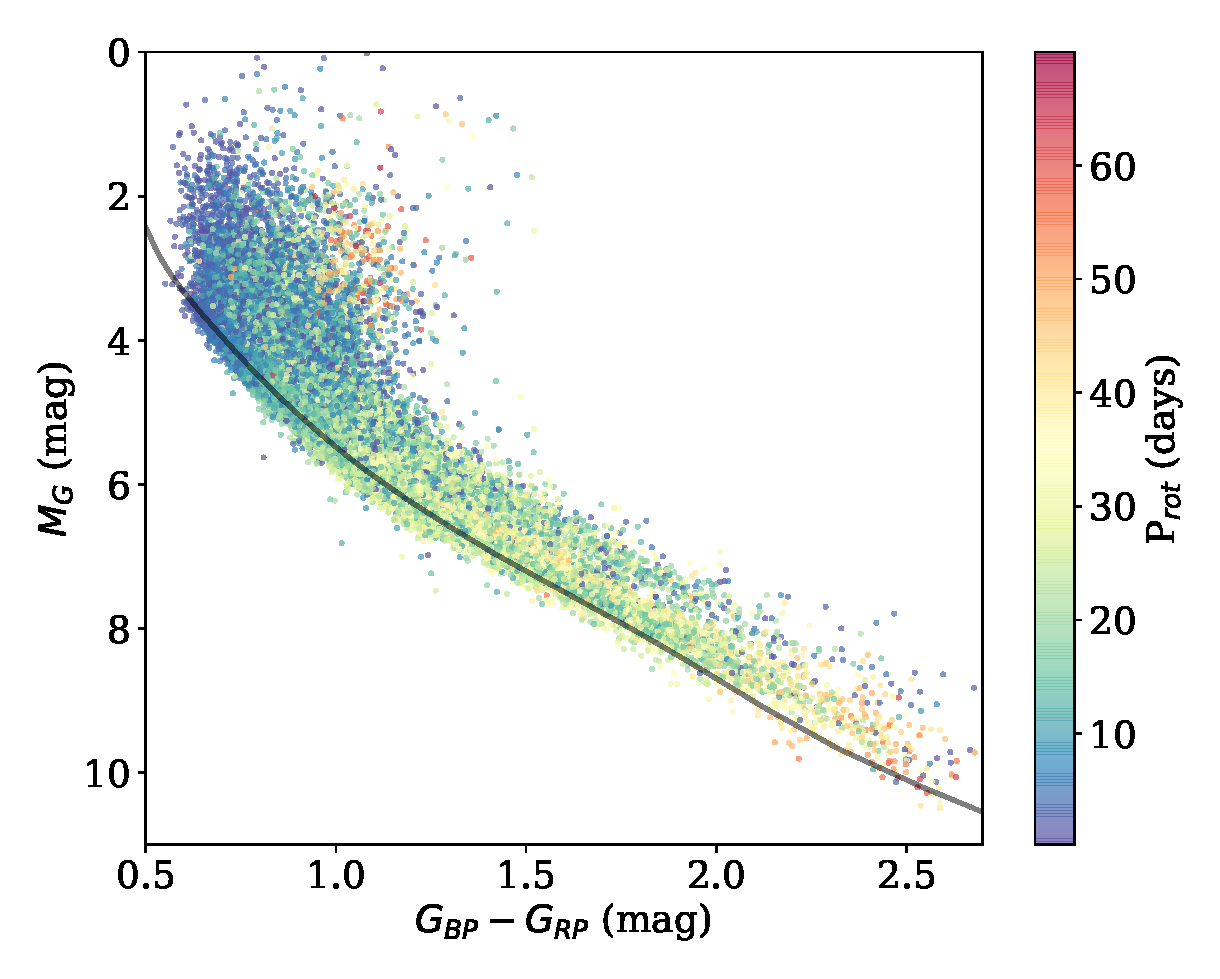
\includegraphics[width=3.6in]{../figures/cmd}
\caption{
Color--magnitude diagram for 30,305 \Kepler stars from the \citet{mcquillan2014} sample that are included in Gaia DR2, colored by their measured rotation period. For reference we show a $10^9$ year MIST isochrone (black line) used to select likely main sequence, single stars (black line). A track of binary  stars is apparent $\sim$0.75 mag above the main sequence. As in \citet{davenport2017}, we find significant contamination of the rotation period sample for bluer stars by sub-giants.}
\label{fig:cmd}
\end{figure}




%%%%%%%%%%%%%%%%%%%%%%
\section{Selecting Main Sequence Stars}

As in \citet{davenport2017}, the color--magnitude diagram in Figure \ref{fig:cmd} shows many of the bluer stars in the \citet{mcquillan2014} sample are located significantly above the main sequence. These are likely subgiant stars, which do not follow the main sequence stars spin-down evolution \citep[e.g.][]{donascimento2012, van-saders2013}. Since \citet{davenport2017} found subgiants could obscure the rotation period bimodality for G dwarfs, these must be excluded from our analysis, but we encourage future studies to explore the wealth of angular momentum evolution data from these most-main sequence objects.

Beyond the subgiant contamination, we also see a secondary population of stars in a parallel track $\sim$0.75 mag above the normal main sequence, which are attributed to unresolved binary star systems. This pile-up above the main sequence occurs due to unresolved equal-mass (or nearly equal-mass) field binaries, and was seen in the {\em Gaia} DR1 data as well \citep{anderson2017}. Since these systems may have experienced tidal evolution that could significantly impact their rotation evolution \citep[e.g.][]{lurie2017}, we must also remove these from our analysis. Though we do not explore the binary population in any detail here, this sample (perhaps with radial velocity follow-up) may provide useful insight into the tidal evolution of binary stars, and are good targets for characterizing binary star system properties. We also note a small number of systems above the even the equal-mass binary main sequence track, which could be due to unresolved triple star systems.

We use an isochrone from the Mesa Isochrones and Stellar Tracks suite \citep[MIST;][]{MIST} to choose likely main sequence stars in Figure \ref{fig:cmd}. Our favored model to represent the main sequence in this study had [Fe/H] = +0.25 and an age of $10^9$ years, and was chosen by-hand. Single, main sequence stars were selected in a region spanning 0.1 mag fainter and 0.4 mag brighter than the MIST isochrone, resulting in a final sample  of 16,248 stars for analysis of their rotation period distributions.







%%%%%%%%%%%%%%%%%%%%%%
\section{Tracing the Period Bimodality}
Using this sample of likely single, main sequence stars from \Kepler and {\em Gaia}, we are able to explore the distribution of rotation periods for stars as a function of their distance. The rotation period bimodality in \Kepler stars previously only detected for stars within $\sim$300 pc of the Sun due to the limits of available parallax data. Now with {\em Gaia} DR2, our sample of main sequence star with measured rotation periods in \Kepler extends out to over 2 kpc.

In Figure \ref{fig:color_period} we present the period--color diagram for our sample of stars, split into six bins of projected distance. The first panel (0--350 pc) effectively reproduces the results of \citet{davenport2017} for bluer stars and \citet{mcquillan2014} for the redder stars. A gap in the observed rotation periods as a function of color is seen, at a period of approximately 5 days for $G_{BP}-G_{RP}\approx1$, 20 days for $G_{BP}-G_{RP}\approx2$, and increasing towards 30 days for the reddest stars in our sample. This gap corresponds with a line of approximately constant age, consistent with a gyrochrone with age $\sim$600 Myr \citep{davenport2017}. 


\begin{figure*}[]
\centering
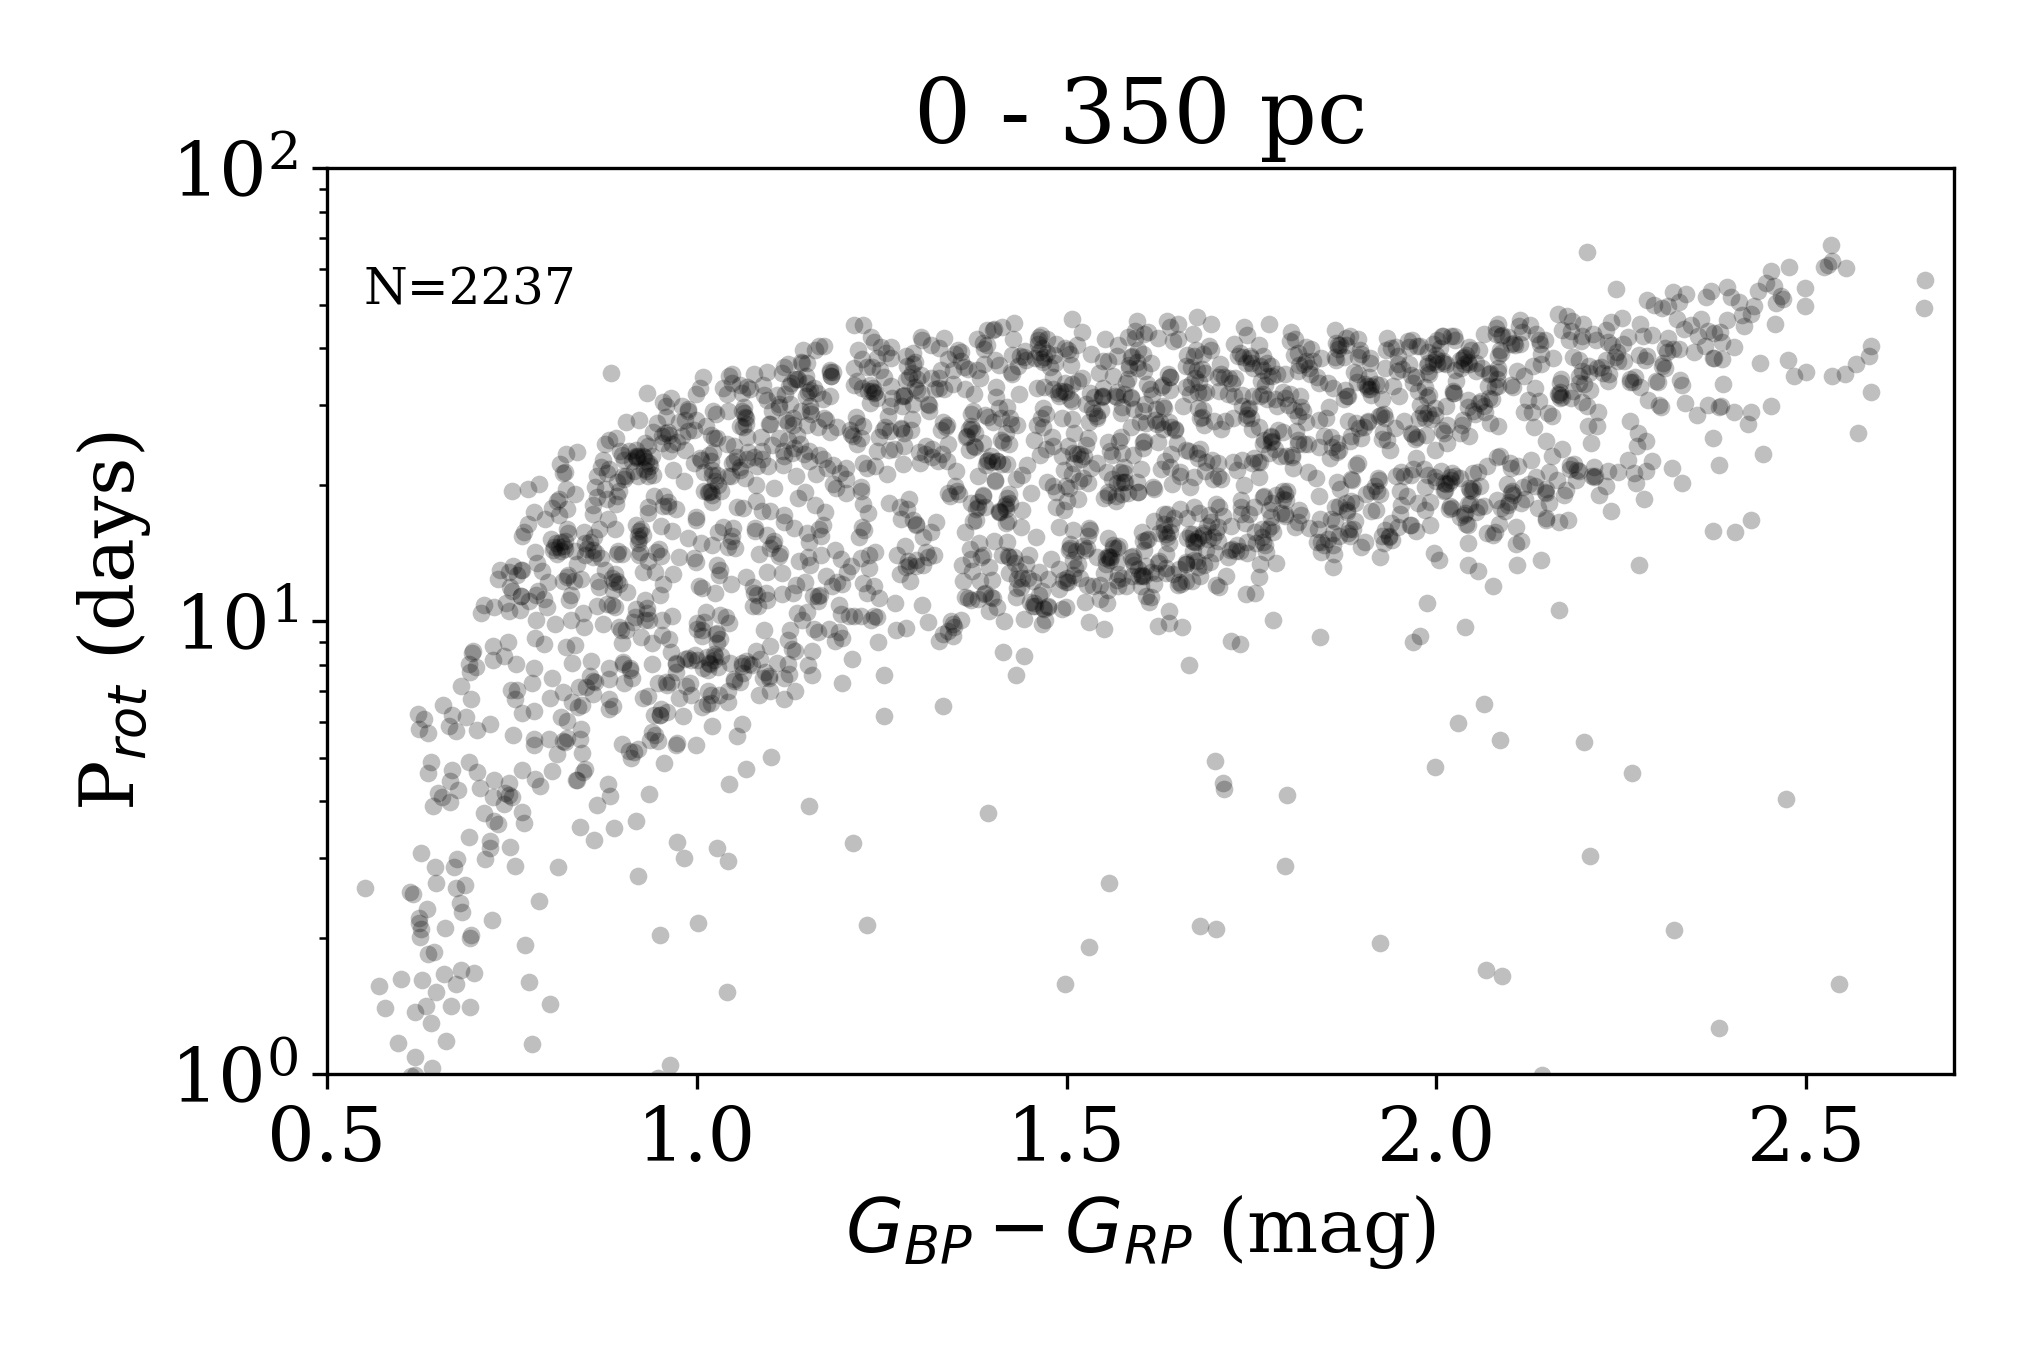
\includegraphics[width=3.5in]{../figures/rot_dist_0}
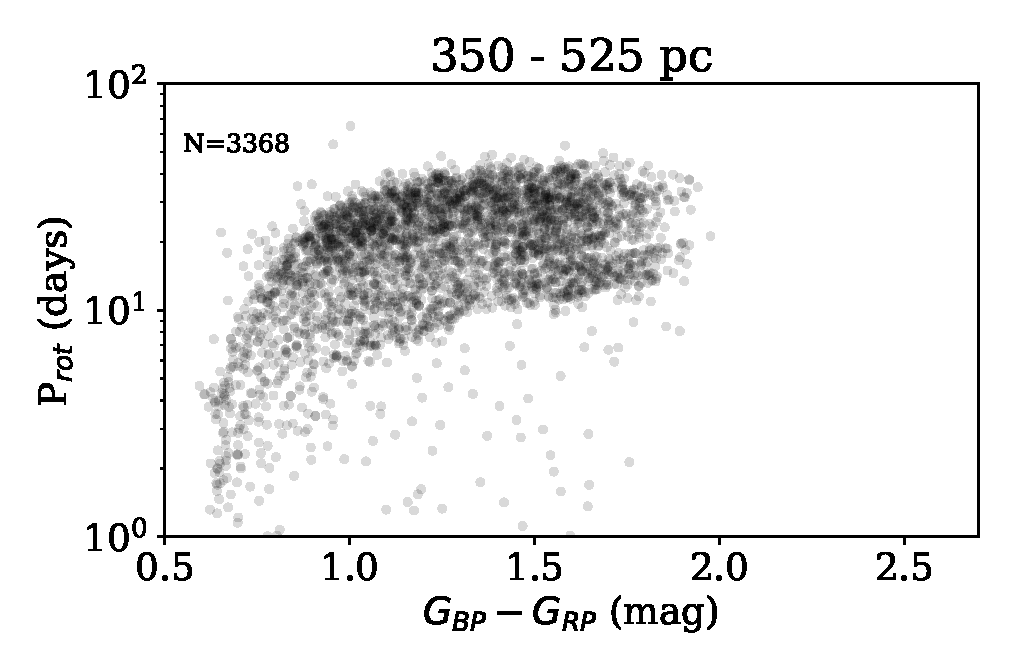
\includegraphics[width=3.5in]{../figures/rot_dist_350}
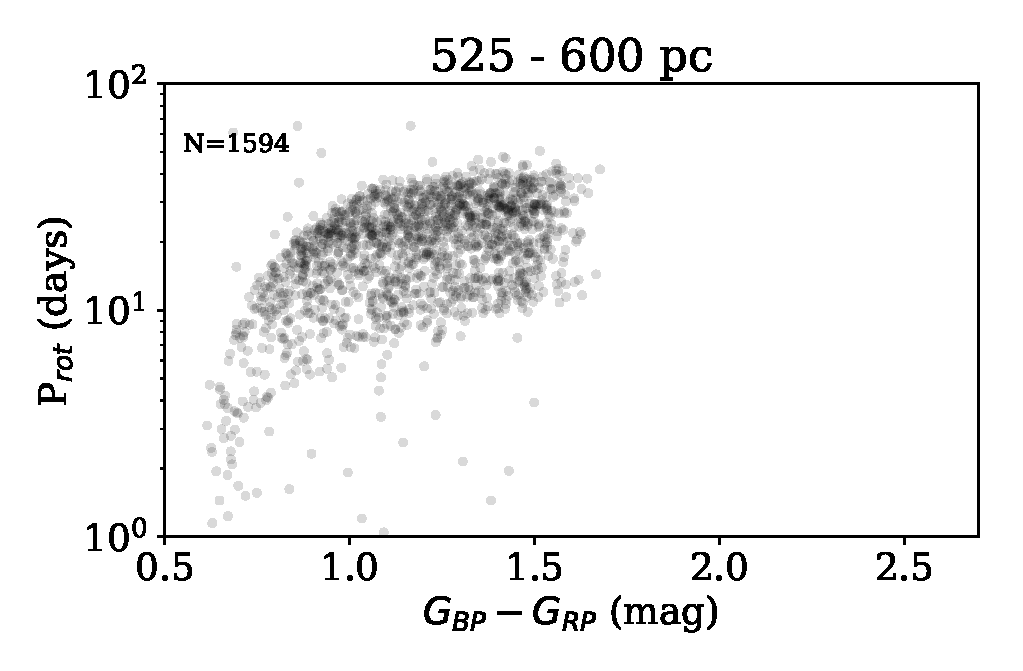
\includegraphics[width=3.5in]{../figures/rot_dist_525}
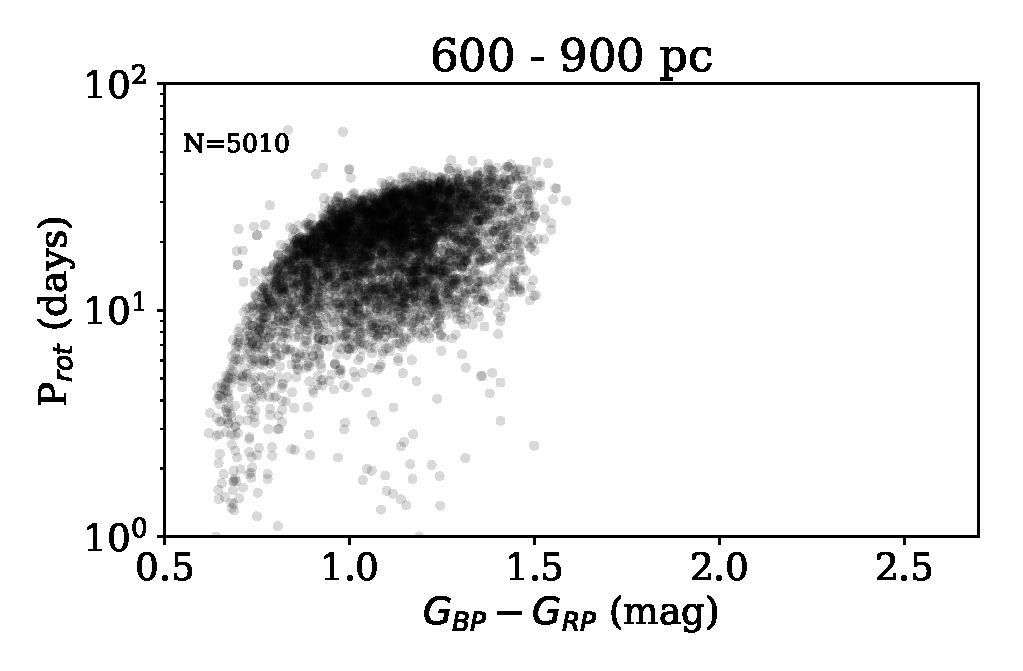
\includegraphics[width=3.5in]{../figures/rot_dist_600}
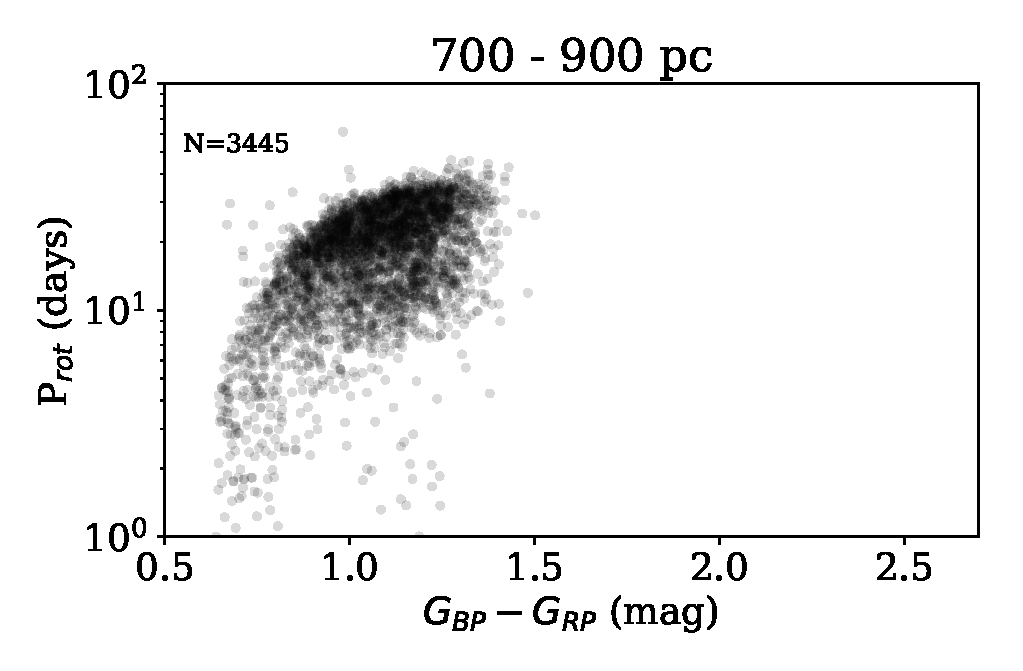
\includegraphics[width=3.5in]{../figures/rot_dist_700}
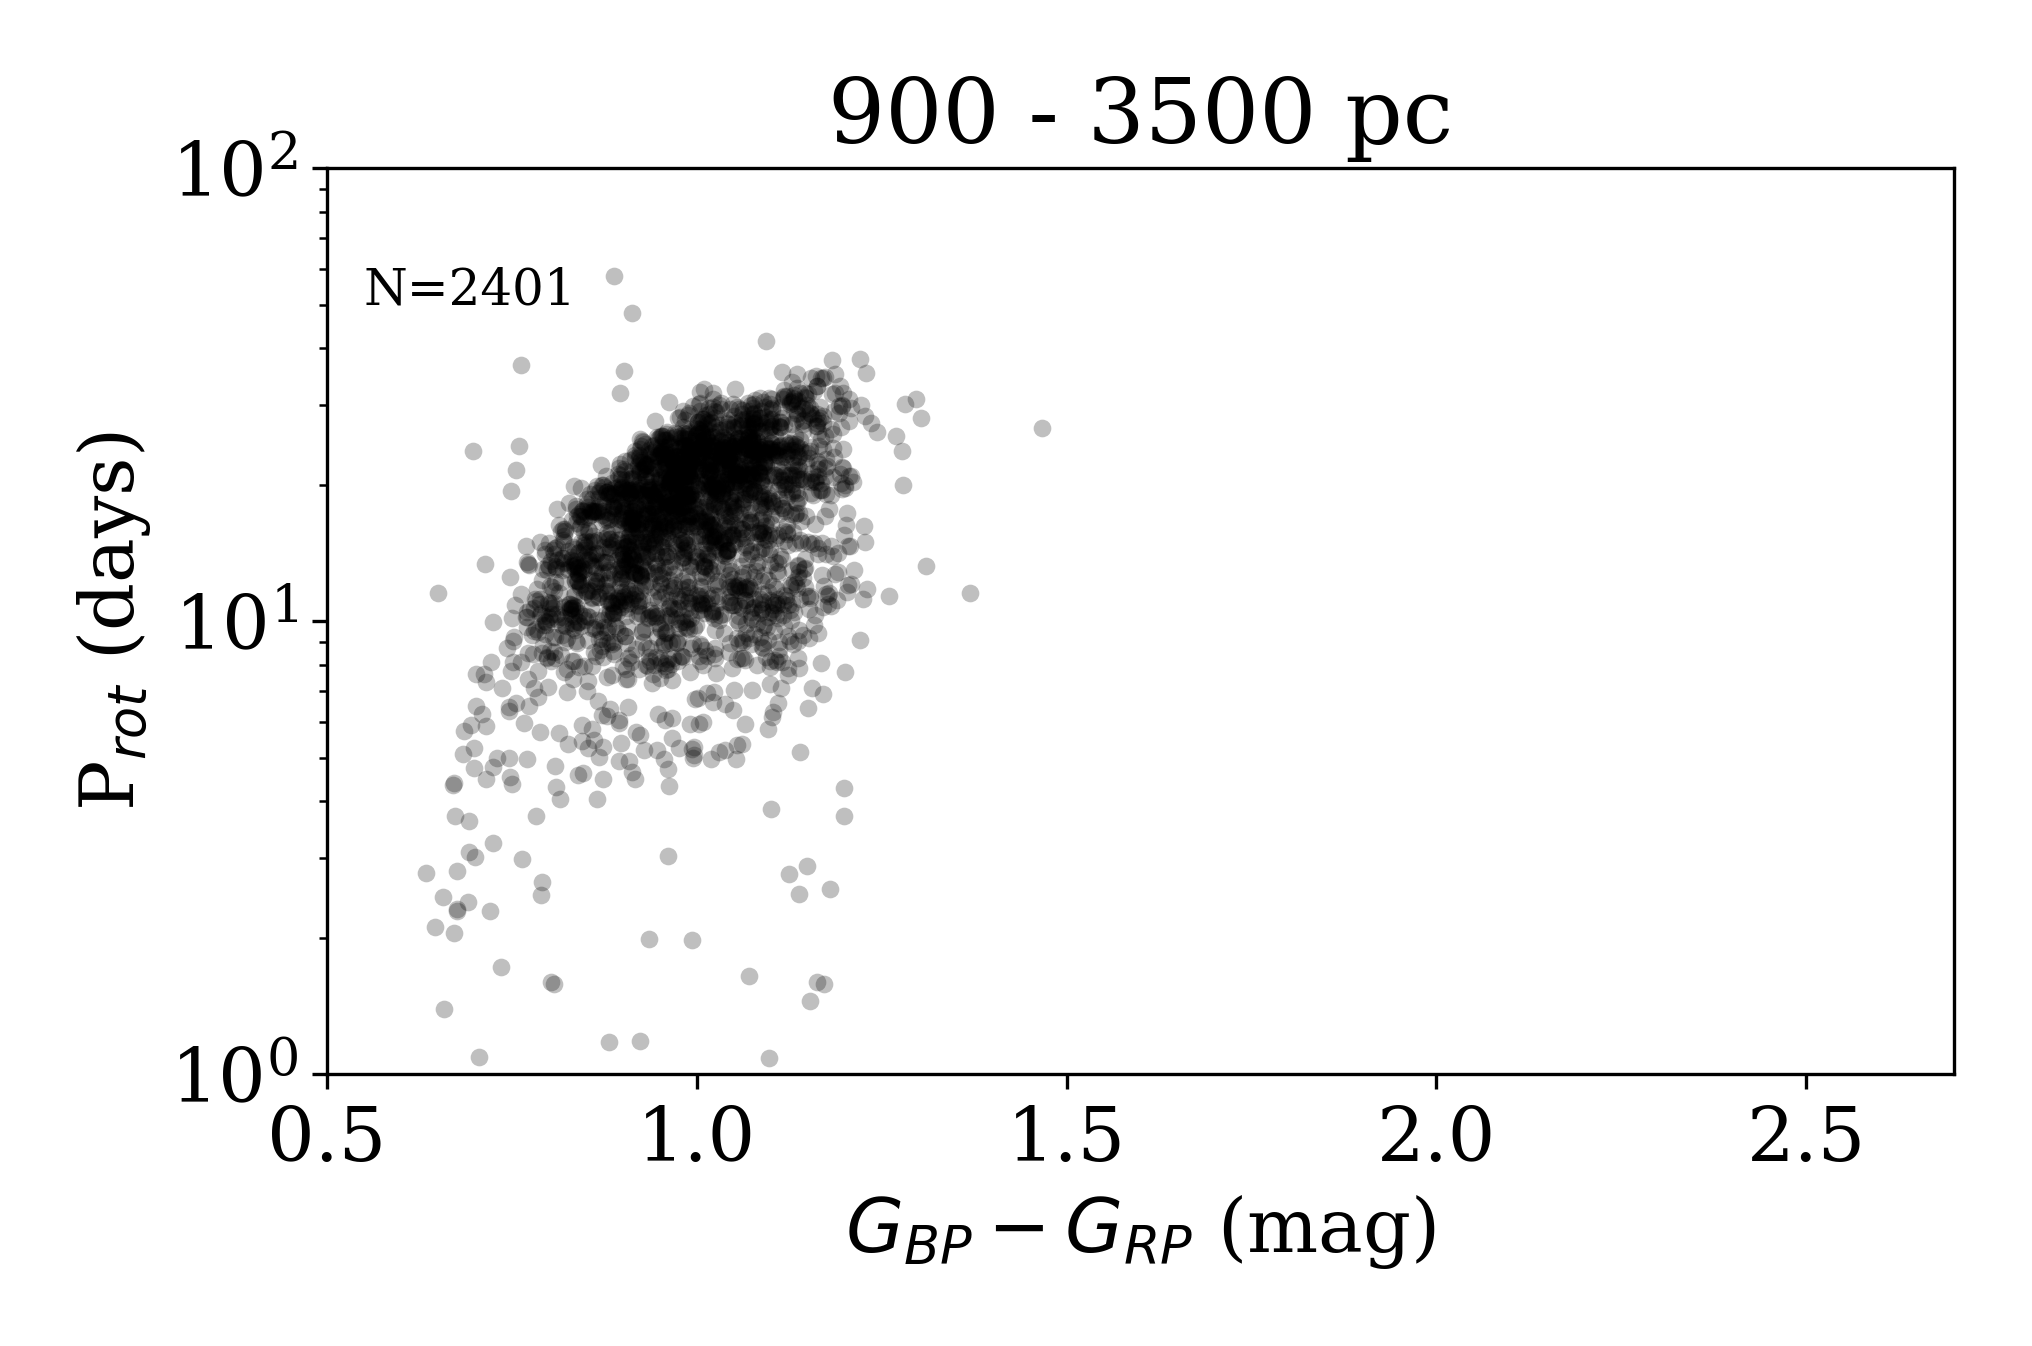
\includegraphics[width=3.5in]{../figures/rot_dist_900}
\caption{Color--period diagrams for our sample of likely main sequence stars, divided into six bins of distance. Our nearest bin (within 350pc) is effectively the distance analyzed in \citet{davenport2017} using Gaia DR1, and clearly shows the rotation period bimodality for the entire sample. The brighter magnitude limit of the \Kepler sample results in redder (fainter) stars missing in our further distance bins. The rotation period bimodality can be seen in the 350-525 pc bin, but is not found in the bluer stars at further distances.
}
\label{fig:color_period}
\end{figure*}


The bimodality is still apparent in the second distance bin (350--525 pc), clearly visible in the redder stars, but seems to fade in the final three bins. Other structures in the period distributions are visible, however. For example, a thin sequence of stars with rotation periods near 10 days is faintly visible in the most distant bin (900--2500 pc) for stars with colors of $0.8<G_{BP}-G_{RP}<1.2$. This feature is due to the 1 Gyr open cluster NGC 6811 in the \Kepler field \citep{meibom2011}, whose distance is $\sim$1100 pc \citep{sandquist2016}.


To better illustrate the evolution of rotation periods for all the stars between distance bins, in Figure \ref{fig:per_hist} we follow \citet{davenport2017} and subtract the rotation period of a 600 Myr gyrochrone. As no published gyrochronology model yet exists that has been tuned to the {\em Gaia} photometric colors, we adopt the same gyrochronology model of Eqn. 2 from \citet{meibom2009} used by \citet{davenport2017} to approximately trace the rotation period gap at 600 Myr as a function of $B-V$ color. We convert stars from the observed {\em Gaia} $G_{BP}-G_{RP}$ color to $B-V$ using the same 1 Gyr MIST isochrone model used to define the main sequence in Figure \ref{fig:cmd} above. 

Our sample naturally becomes biased towards the bluer (brighter) stars as we reach larger distances. Since bluer stars have more rapid rotation and more dramatic period evolution, gyrochronology models are ``bent'' strongly for these stars, and thus the period bimodality (or other structures) become difficult to distinguish. \citet{davenport2017} used an ad-hoc modification of the gyrochrone model for the hottest stars to illustrate the existence of the period bimodality. However, in Figure \ref{fig:per_hist} we limit our analysis to stars with $0.8<B-V<1.5$ (approximately $0.9<G_{BP}-G_{RP}<2.2$, or $0.9>M_\odot> 0.5$), where the gyrochrone is most flat as a function of color. This color range was chosen to ensure ample stars were available in each distance bin, but without having to use the ad-hoc gyrochrone model correction from \citet{davenport2017}.

Figure \ref{fig:per_hist} shows clearly that for the rotation period bimodality dominates for the nearest stars

\begin{figure}[]
\centering
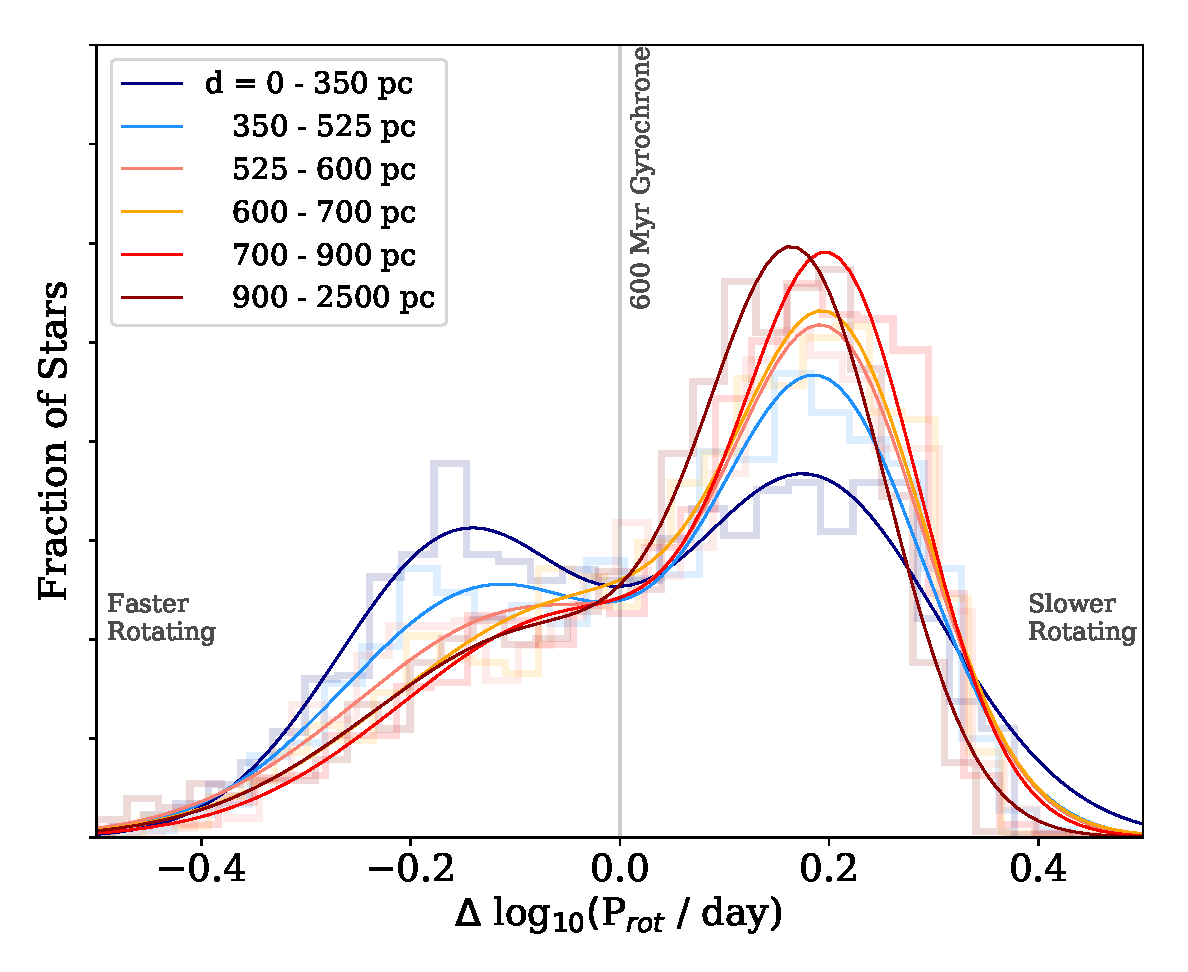
\includegraphics[width=3.5in]{../figures/delta_per_2gauss}
\caption{Histograms of the log rotation periods after a 600 Myr gyrochrone was subtracted for stars in the same six distance bins shown in Figure \ref{fig:color_period} (faint lines). Two-gaussian models were fit to each histogram (bold lines). 
The period bimodality for stars within 350 pc has two nearly equal peaks similar to those found in \citet{davenport2017}, at -0.15 and +0.18 dex. The fast rotating peak (left side) declines sharply at further distances.
}
\label{fig:per_hist}
\end{figure}




\Kepler field has a central Galactic latitude of $b\sim13.5^\circ$, pointing slightly above the Galactic midplane. 
these distance bins reach approximate distances above the galactic midplane of $\sim$60 pc in the nearest bin, to nearly 800 pc in the furthest bin, therefore spanning a large range in apparent age and possible star formation history
%  61.70587735  102.55881602  120.06721831  190.10082747  797.0587735  pc
Both galaxy formation simulations \citep{ma2017} and observations of stars in the nearby Milky Way \citep{xiang2017} indicate that height above the midplane correlates strongly with the median ages for stars. However, since the \Kepler field is not very upwardly inclined, we not reaching significant {\it heights} above the plane. therefore we think the localization of the period bimodality is related to an age feature that is localized within the disk near the Sun, not representative of the total star formation history of our galaxy.

\citet{lewis2015} for example show lots of variation in SFH in 100pc bins for M31




%\clearpage
%%%%%%%%%%%%%%%%%%%%%%
\section{Recalibrating Stellar Evolution Models}

\begin{figure*}
\centering
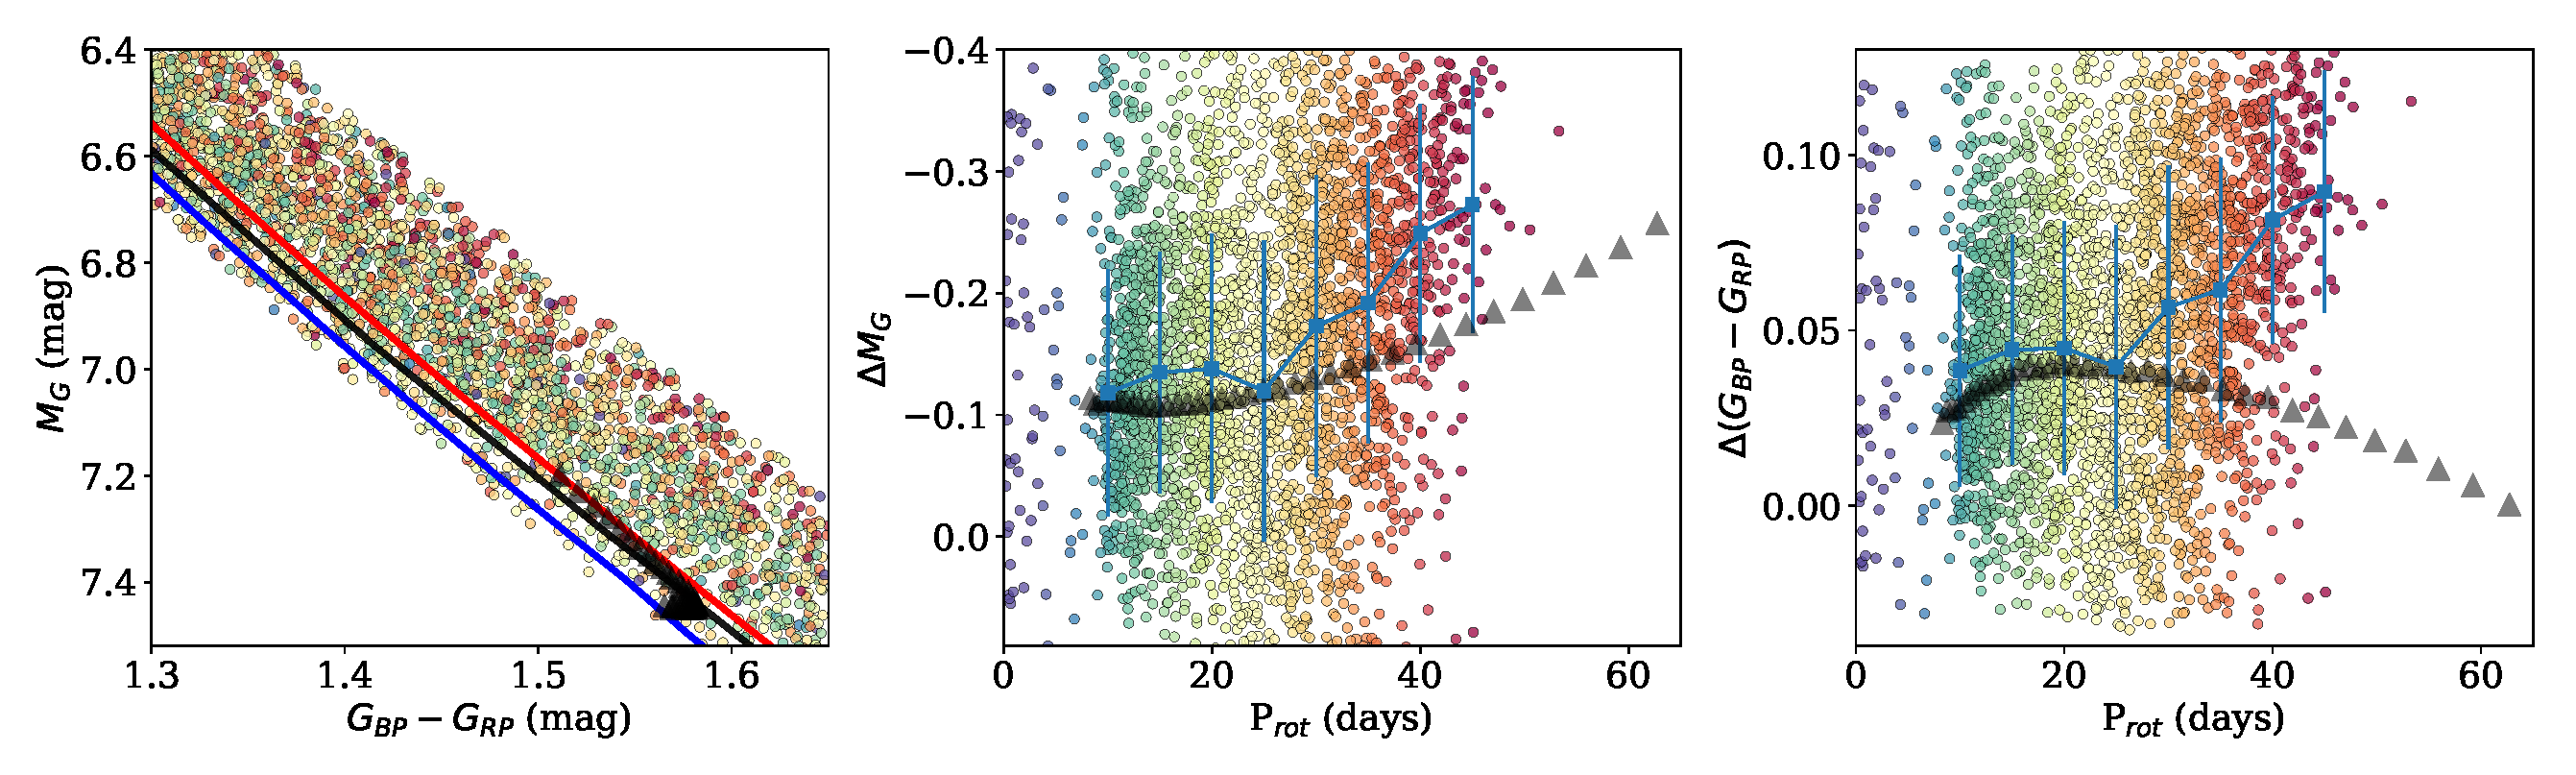
\includegraphics[width=6in]{../figures/cmd_zoom}
\caption{
Left: Enlarged portion of the color--magnitude diagram from Figure \ref{fig:cmd} in a region centered near $\sim$0.75 M$_\odot$, with stars are colored by their measured \Kepler rotation periods from \citet{mcquillan2014}.
MIST isochrones at ages of $10^8$, $10^9$, and $10^10$ yr are shown for comparison (blue, black, and red lines). The predicted evolution of a 0.7 M$_\odot$ star is highlighted (black triangles). %The main sequence shows significant scatter, as well as a gradient in rotation period with slower rotators preferentially above the main sequence. 
Right: Difference in $M_G$ from the $10^9$ yr MIST isochrone as a function of rotation period (point color again indicates rotation period, as in Left panel). Blue squares show an increase in the median $M_G$ offset in bins of increasing rotation period. Error bars shown are the standard deviation of $\Delta M_G$ in each bin. The 0.7 M$_\odot$ star brightness evolution is shown as a function of rotation evolution from \citet{meibom2009} (black triangles).
}
\label{fig:cmd_zoom}
\end{figure*}



A subtle feature that we noticed in Figure \ref{fig:cmd} is the apparent color gradient (i.e. rotation period gradient) between the single and binary star main sequence populations. In Figure \ref{fig:cmd} this appears as a yellow stripe (i.e. rotation periods of 30-40 days) between these blue-green sequences for systems with colors of $G_{BP} - G_{RP} \approx 1.5$. To exaggerate this feature, we have reproduced a portion of our color--magnitude diagram focused on the main sequence near this stellar color in the left panel of Figure \ref{fig:cmd_zoom}. A clear color gradient is present, with red points (slower rotators) appearing preferentially above the main sequence.
The right panel of Figure \ref{fig:cmd_zoom} concretely demonstrates a correlation between the measured rotation period and the vertical offset (i.e. absolute magnitude) from the $10^9$ year MIST isochrone. Slower rotating stars are apparently brighter at a given stellar color.

We interpret this observation as being due to the increase in luminosity of stars across their main sequence lives, coupled with the angular momentum loss that underpins gyrochronology. Indeed, the sequence of MIST isochrones shown in Figure \ref{fig:cmd_zoom} with ages of $10^8$, $10^9$, and $10^10$ years clearly predicts an increase in brightness of the main sequence over time. 

indeed, 0.7solarmass star traced over its life in both panels doesnt quite make sense. 
inverting CMD into precise ages w/ Gaia beyond scope of this work, but this figure suggests the MS is too wide given a reasonable age range. consider: younger stars, presumably more metal rich, should be redder, moving in the wrong direction to the affect we see here. more stellar masses and careful work needed... vertical spread in this parameter space is OK for a star, but maybe some color impact we not considering.... hmm.

however, looking at 0.7M period vs lum evolution, we see that the period seems to also drop off too rapidly compared to a model. combining the MM09 spin-down formulae for a 0.7M star, with the MIST isochrone evolution, we see  the period range should go out to 60--80 days to get the right amplitude offset. That implies that at a given age (or vertical offset), the stars are rotating {\it faster} than expected. this is similar to the broken spin-down model suggested by \citep{van-saders2016}, and is potentially the first confirmation of this observation.







%%%%%%%%%%%%%%%%%%%%%%
\section{Discussion}
%
%Using a combination of data from \Kepler and Gaia DR1, I have explored the rotation period distribution for 440 nearby main sequence stars. A bimodal rotation period distribution has been found in stars with temperatures ranging from 5000 K to 6500 K. This feature matches that found in cooler stars from \Kepler, but was only revealed thanks to the enhanced ability to distinguish dwarfs from subgiants using Gaia data. 
%A tenuous difference in the TGAS total proper motion for stars in the fast and slow rotating groups is found, which is in agreement with the findings for cool stars by \citet{mcquillan2013}.
%
%While a definitive explanation for this period bimodality has not been reached, the findings to date seem to favor stellar ages as the cause. In this scenario the star formation history for nearby stars would be dominated by two epochs of star formation, one short event centered at a few hundred Myr, and one long event centered at a few Gyr (slightly younger than the Sun). It is also worth noting that the space volume probed by the TGAS sample investigated here is very similar to that covered by the temperature-selected cool star sample in \citet{mcquillan2013}. The median parallax distance for stars in this work is 285 pc, while the median isochrone distance for the K and M dwarfs is $\sim$216 pc. This points to the period distribution being a localized age artifact. 
%Determining how localized this age distribution is, and if it can be confirmed for stars across the HR diagram including giants, is a key goal for future Gaia data releases.
%
%
%The period bimodality may yet be a manifestation of the ``Vaughan-Preston'' gap observed in chromospheric activity indicators from solar type stars. Such a feature has also been discussed for rotating stars by \citet{kado-fong2016}. Given that the mass range for the bimodality explored here and in \citet{mcquillan2014} covers stars with solar-type dynamos (those having a tachocline, late F through early M) such a model cannot be fully ruled out at this time. Though there have been many rotation studies for cool stars \citep[e.g.][]{irwin2011,newton2016,stelzer2016} too few rotation periods have been measured for stars across the ``fully convective boundary'' ($T_{eff}<3000$ K, spectral type $\sim$M4) to tell if the bimodal period feature continues to cooler temperatures, which would support the age distribution model. 
%If the bimodality is due to stars crossing a phase of rapid angular momentum evolution, we would expect to see it in stellar clusters at or near the critical age. The lack of this feature in the clusters observed to date could be due to no cluster being close enough to the critical age, which the gyrochrone in Figure \ref{fig:gyro} shows is near 600 Myr. Further studies of rotation periods for stars in intermediate age open clusters (e.g. the Hyades) may help solve this mystery \citep[e.g.][]{douglas2014}.
%
%Finally, this exploratory work has highlighted the utility of using astrometric data from Gaia combined with detailed light curve statistics from \Kepler to reveal hidden substructure in the properties of field stars. Looking forward to the astrometric precision of future Gaia data releases, this combination will be effective at separating dwarf stars from subgiants for nearly the entire \Kepler and K2 databases, and enable accurate age maps for field stars.



%%%%%%%%%%%%%%%%%
\acknowledgments

JRAD is supported by an NSF Astronomy and Astrophysics Postdoctoral Fellowship under award AST-1501418. 

This work made use of the \url{gaia-kepler.fun} crossmatch database, created by Megan Bedell.

This project was developed as part of the 2018 NYC Gaia Sprint, hosted by the Center for Computational Astrophysics at the Simons Foundation in New York City.


This work has made use of data from the European Space Agency (ESA) mission
{\it Gaia} (\url{https://www.cosmos.esa.int/gaia}), processed by the {\it Gaia}
Data Processing and Analysis Consortium (DPAC,
\url{https://www.cosmos.esa.int/web/gaia/dpac/consortium}). Funding for the DPAC
has been provided by national institutions, in particular the institutions
participating in the {\it Gaia} Multilateral Agreement.



\bibliography{/Users/james/Dropbox/references}

\end{document}
